% setup
\documentclass[12pt,a4paper]{article}
\usepackage[utf8]{inputenc}
\usepackage[german]{babel}
\usepackage{csquotes}
\usepackage[T1]{fontenc}
\usepackage{amsmath}
\usepackage{amsfonts}
\usepackage{amssymb}

%matrices
\usepackage{blkarray}

%figures & images
\usepackage{graphicx}
\usepackage{subcaption}

%utils
\usepackage{color}
\usepackage{hyperref}

% Bibliographie
\usepackage[backend=biber,style=alphabetic,citestyle=authoryear]{biblatex}
\bibliography{Thesis}
\usepackage[nottoc]{tocbibind}


% todo command
\newcommand\todo[1]{\textcolor{red}{#1}}

% Document Infos
\author{Amandus Stefan Butzer}
\title{Erstellung eines Routing-Profils auf Basis von OpenStreetMap-Daten für Feuerwehrfahrzeuge}
\date{\today}

\begin{document}
\begin{titlepage}
\begin{center}

	{\scshape\LARGE Ruprecht-Karls-Universität Heidelberg\par}
	\vspace{1.5cm}
	{\LARGE\bfseries Bachelorarbeit\par}
	\vspace{2cm}
	{\Huge\bfseries Erstellung eines Routing-Profils auf Basis von OpenStreetMap-Daten\par für Feuerwehrfahrzeuge\par}
	\vspace{2cm}
	{\Large\itshape Amandus Stefan Butzer\par}
	\vspace{2cm}
	{\large Fakultät für Chemie und Geowissenschaften \par Geographisches Institut \par Abteilung Geoinformatik\par}
	\vfill
	{Betreut von\par Prof. Dr. Alexander Zipf}

	\vfill

% Bottom of the page
	{\large \today\par}
\end{center}
\end{titlepage}

\newpage

{\centering\section*{Zusammenfassung}}
\todo{Deutsche Kurzfassung}\par
Lorem ipsum dolor sit amet, consetetur sadipscing elitr, sed diam nonumy eirmod tempor invidunt ut labore et dolore magna aliquyam erat, sed diam voluptua. At vero eos et accusam et justo duo dolores et ea rebum. Stet clita kasd gubergren, no sea takimata sanctus est Lorem ipsum dolor sit amet. Lorem ipsum dolor sit amet, consetetur sadipscing elitr, sed diam nonumy eirmod tempor invidunt ut labore et dolore magna aliquyam erat, sed diam voluptua. At vero eos et accusam et justo duo dolores et ea rebum. Stet clita kasd gubergren, no sea takimata sanctus est Lorem ipsum dolor sit amet.

\newpage
{\centering\section*{Abstract}}
\todo{Abstract in Englisch}
Lorem ipsum dolor sit amet, consetetur sadipscing elitr, sed diam nonumy eirmod tempor invidunt ut labore et dolore magna aliquyam erat, sed diam voluptua. At vero eos et accusam et justo duo dolores et ea rebum. Stet clita kasd gubergren, no sea takimata sanctus est Lorem ipsum dolor sit amet. Lorem ipsum dolor sit amet, consetetur sadipscing elitr, sed diam nonumy eirmod tempor invidunt ut labore et dolore magna aliquyam erat, sed diam voluptua. At vero eos et accusam et justo duo dolores et ea rebum. Stet clita kasd gubergren, no sea takimata sanctus est Lorem ipsum dolor sit amet.

\newpage
\section*{Erklärung}
\vspace{1cm}
Hiermit versichere ich, dass ich die vorliegende Bachelorarbeit selbstständig verfasst, noch nicht anderweitig zu Prüfungszwecken vorgelegt, keine anderen als die angegebenen Quellen oder Hilfsmittel benutzt, sowie wörtlich und sinngemäße Zitate als solche gekennzeichnet habe.\par
\bigskip

{\flushleft Heidelberg den \today } {\hfill .....................................\par}
{\hfill (Unterschrift)}

\newpage
\tableofcontents

\newpage
\listoffigures


\newpage
\section{Einleitung}

\subsection{Motivation}
Zum Zeitpunkt der Erstellung dieser Arbeit ist der Verfasser in der Geoinformatik Abteilung des Geographischen Instituts der Ruprecht-Karls-Universität Heidelberg als wissenschaftliche Hilfskraft des openrouteservice (ORS) tätig. Der ORS bietet neben Geocoding, Routing und Location Service auch einen Isochrone Service an. \par
\bigskip
Immer wieder wurden Anfragen bezüglich Erreichbarkeitsanalysen aus dem Rettungs- und Brandschutzwesen erhalten. Für Polizei, Rettungsdienst und Feuerwehr geht es vor allem um das Einhalten amtlich vorgegebener Hilfsfristen. Diese stellen eine bedeutsame Eigenschaft für die Planung und Qualität der Einsätze von Feuerwehr und Rettungsdienst dar.\par
Der Brandschutz ist im Gegensatz zum Rettungsdienst eine kommunale Aufgabe und unterliegt nur in manchen Bundesländern bestimmten Standards (vgl.{bedarfsplan}). Daher bedienen sich diese Organisationen unterschiedlicher Hilfsmittel um Bedarfspläne für ihren Standort zu erstellen.
\medskip

Da mit dem Isochrones-Service des ORS Erreichbarkeitsanalysen durchgeführt werden, ist dieser für die Erstellung eines Brandschutzbedarfsplans der Feuerwehr geeignet. Jedoch kann der Dienst in seiner bisherigen Form noch nicht alle erforderlichen Anforderungen für Einsatzfahrzeuge erfüllen.
\vspace{1.2cm}

\textbf{§35 Abs. 1 StVO:}
\begin{quotation}
{\itshape\rmfamily ''Von den Vorschriften dieser Verordnung sind die Bundeswehr, die Bundespolizei, die Feuerwehr, der Katastrophenschutz, die Polizei und der Zolldienst befreit, soweit das zur Erfüllung hoheitlicher Aufgaben dringend geboten ist.''}
\end{quotation}

\vspace{1.2cm}

Dieser kurze Absatz der Straßenverkehrs-Ordnung ermöglicht es Einsatzfahrzeugen sich unter Benutzung von Martinshorn und Blaulicht über jede Vorschrift im Straßenverkehr hinwegzusetzen. Im Notfall hat das schnellste Erreichen des Zielorts eine höhere Priorität als Geschwindigkeitsbegrenzungen oder Fahrverbote. Bisher gibt es trotz einer großen Anzahl an Routing-Services keinen, der diese Tatsache berücksichtigt. 


\subsection{Zielsetzung}
Das Ziel dieser Arbeit ist in Kooperation mit der Freiwilligen Feuerwehr Lützelburg zu Ermitteln, bis zu welchem Grad diese Notstandsvollmachten im Ernstfall in Anspruch genommen werden können. Auf Basis dieser Informationen soll dann ein Emergency-Routing-Profil (dt.:\textit{emergency} = Notfall) entwickelt werden. Die Implementierung wird aufgrund des Umfangs einer Bachelorarbeit auf eine Fahrzeugklasse der Feuerwehr begrenzt. Allerdings wird bei der Erstellung des Emergency Profils darauf geachtet, dass Erweiterungen für diverse Einsatzfahrzeuge sehr einfach möglich sind.
\vspace{0.5cm}
\begin{flushleft}


Als Basis wird das Profil auf dem Backend des bereits bestehenden Routing Service des ORS aufgebaut. Zusätzlich sollen Java Funktionen implementiert werden, die speziell auf das Emergency Profil zugeschnitten sind. Zur Darstellung wird das ORS Frontend mit Hilfe der Java-Script Programmiersprache angepasst. Dadurch sollen die Ergebnisse in verständlicher und anschaulicher Weise dargestellt werden. 
\todo{(weitere Infos über technic details?)}

\end{flushleft}
\newpage
\section{Theoretische Grundlagen}

Als Grundlage für die Berechnung kürzester Wege wird eine Speicherform aus der Mathematik benutzt, der Graph. 

\subsection{Graphen}

Ein Graph ist ein sehr nützliches Konzept um Objekte und deren Verbindungen untereinander zu modellieren. Die in der Graphentheorie verwendeten Termini belaufen sich dabei auf Ecken (engl: \textit{nodes} oder \textit{vertices}) für Objekte und Kanten (engl: \textit{edges}) für Verbindungen.
(\cite[49]{kurt})

Mathematisch ausgedrückt ist ein Graph G die Funktion aus einer endlichen Eckenmenge V und einer endlichen Kantenmenge E (\cite[4]{theory})

	$$G = (V,E)$$


\begin{figure}[h]
\centering
\begin{subfigure}{0.49\textwidth}
\centering
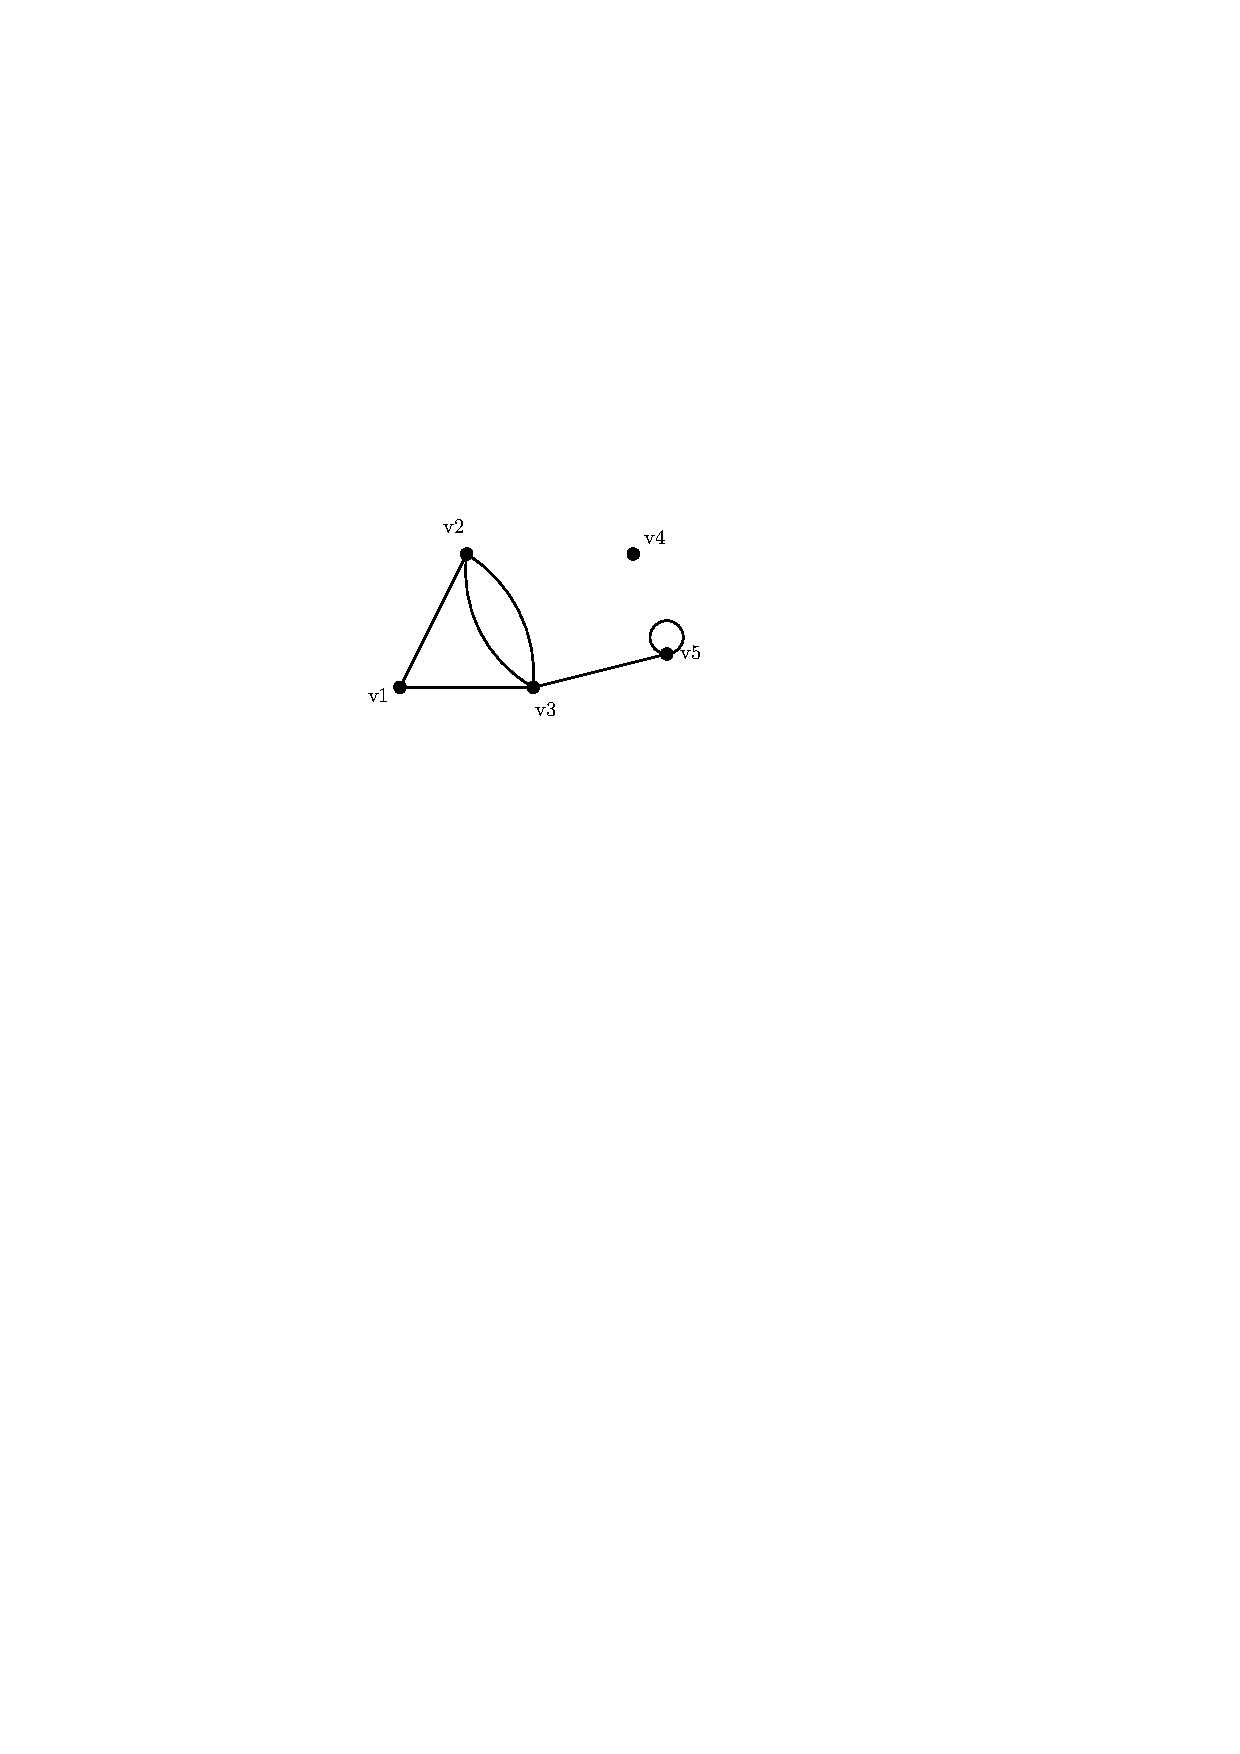
\includegraphics[width = \textwidth]{../media/simpel.pdf} \\
\caption{G}
\label{fig:simple}
\end{subfigure}
\begin{subfigure}{0.49\textwidth}
\centering
{
\begin{blockarray}{cccccc}
  & v1 & v2 & v3 & v4 & v5 \\
\begin{block}{c(ccccc)}
  v1 & 0 & 1 & 1 & 0 & 0 \\
  v2 & 1 & 0 & 2 & 0 & 0 \\
  v3 & 1 & 2 & 0 & 0 & 1 \\
  v4 & 0 & 0 & 0 & 0 & 0 \\
  v5 & 0 & 0 & 1 & 0 & 1 \\
\end{block}
\end{blockarray}
}
\vspace{0.1cm}
\caption{Adjazenzmatrix von G}
\label{mx:simple}
\end{subfigure}
\caption{Ein simpler Graph G}
\label{simpleGraph}
\end{figure}

Der Vorteil von Graphen ist die einfache Darstellung. Dabei werden die Ecken als Punkte und die Kanten als Linien oder Pfeile dargestellt (Abbildung ~\ref{fig:simple}) (\cite[49]{kurt}). Zwischen zwei Ecken können einfache, mehrfache oder keine Kanten bestehen. Darüber hinaus können sie mit sich selbst verbunden sein und eine Schlinge bilden (E). Sind zwei Ecken durch eine Kante verbunden bezeichnet man sie als \textit{adjazent}(benachbart). Ist eine Ecke der Start- oder Endpunkt einer Kante, werden beide Objecte als \textit{inzident} zueinander bezeichnet. Ist eine Ecke zu keiner Kante inzident heißt sie \textit{isoliert}. Ein Graph der keine isolierten Ecken besitzt heißt \textit{zusammenhängend}.(\cite[4--5]{theory}) \par

Computer können Graphen sehr gut verarbeiten, da sich alle Ecken und Kanten in Form von Matritzen speichern lassen. Die Abbildung ~\ref{mx:simple} zeigt an, ob für die jeweilige Eckenkombination des Graphen G eine Kante existiert (1) oder nicht (0). Die Reihen sind die Start- und die Spalten die Endecken. Die '1' in Spalte v1 und Reihe v2 zeigt also an, dass eine Kante von v1 nach v2 existiert. Für ungerichtete Graphen ist eine Kante von v1 nach v2 äquivalent mit einer Kante von v2 nach v1. Daher ist die Adjazenzmatrix für ungerichtete Graphen Spiegelsymmetrisch entlang der Hauptdiagonale ($v1v1 \rightarrow v5v5$). Der Speicherbedarf für eine Matrix folglich halbiert werden, da die eine Hälfte mit der Anderen rekonstruiert werden kann (Abb. ~\ref{mx:iso}). Hat der Graph keine Schlingen, besteht die Hauptdiagonale nur aus Nullen und kann ebenfalls eingespart werden (\cite[19]{algorithms}).

Im folgenden werden nur zusammenhängende Graphen ohne Schlingen betrachtet, da diese für viele Problemstellungen irrelevant sind (\cite[4f]{theory}).

\begin{figure}[h]
\centering
\begin{subfigure}{0.42\textwidth}
\centering
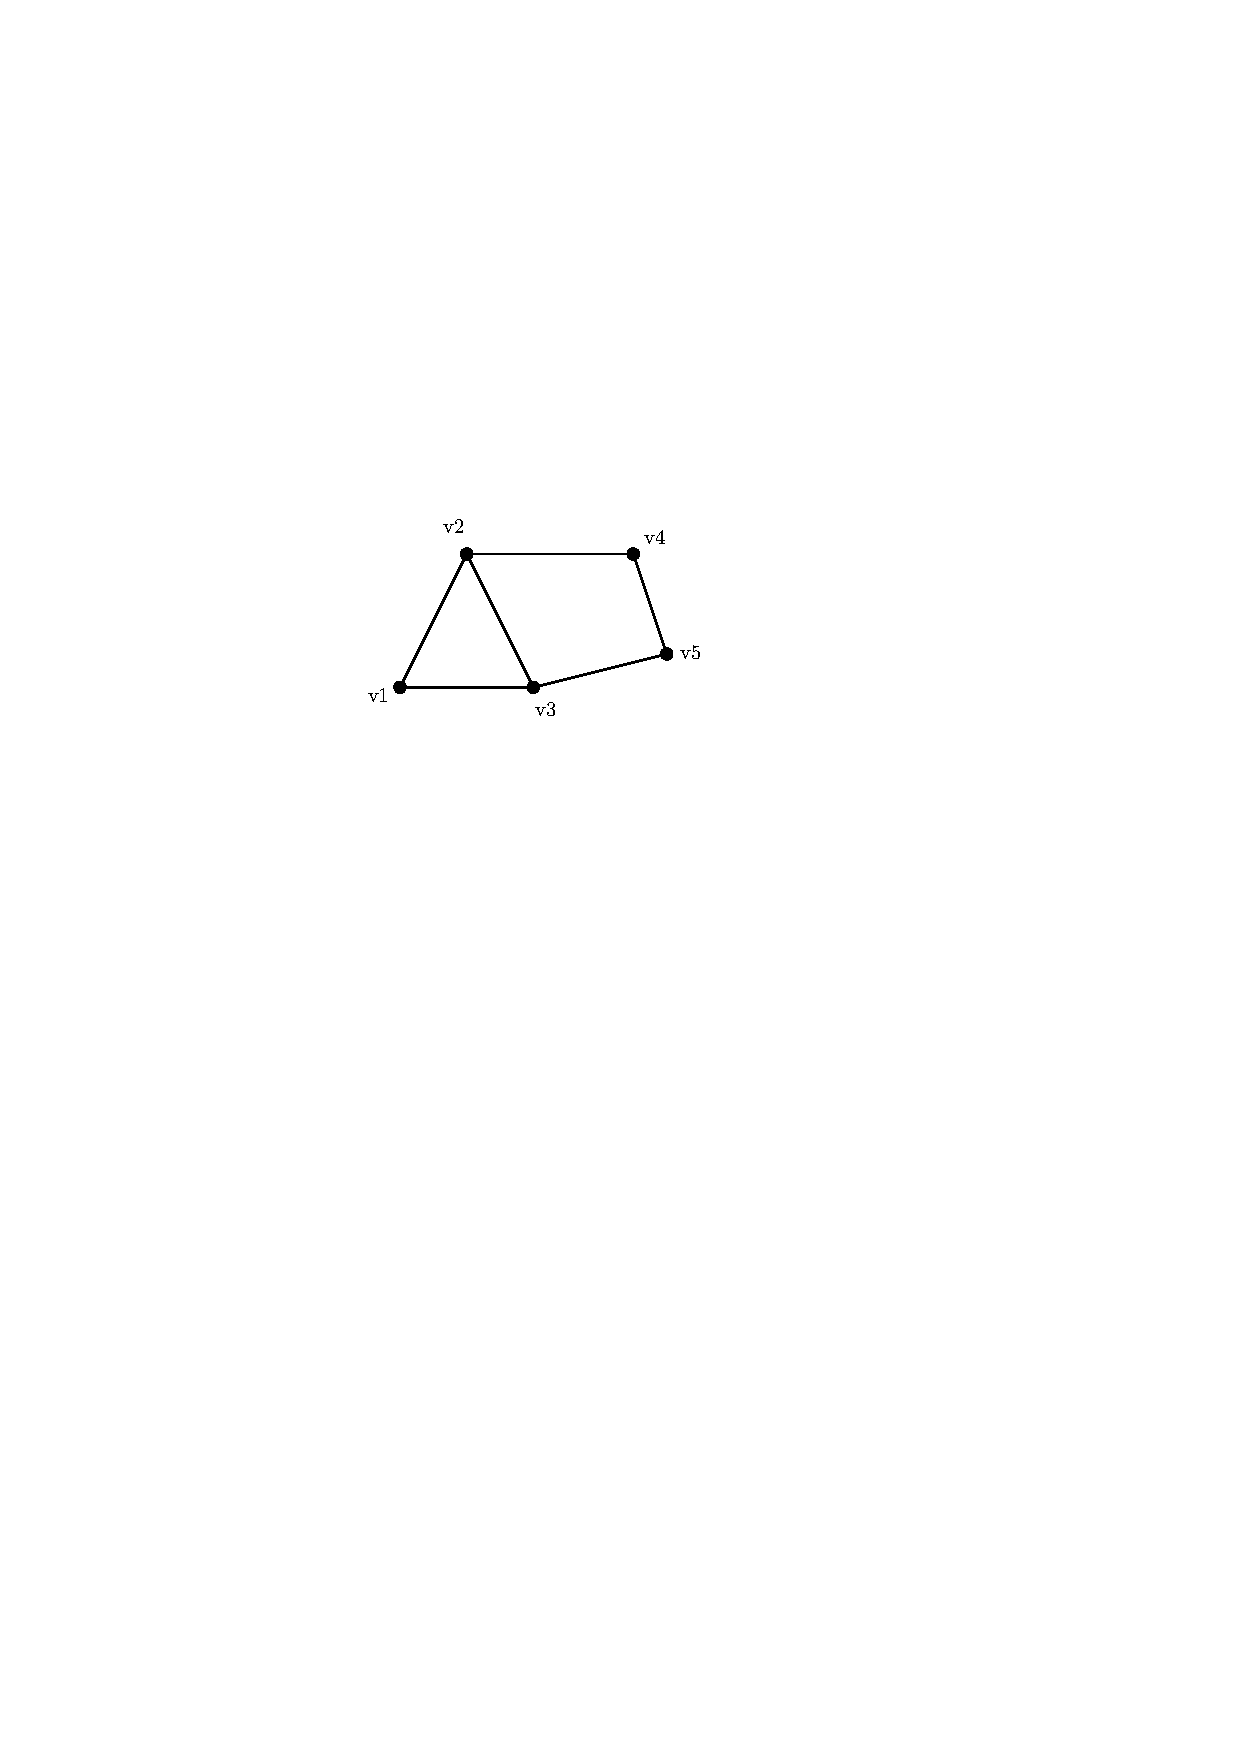
\includegraphics[width = \textwidth]{../media/iso1.pdf} \\
\caption{G}
\label{fig:iso1}
\end{subfigure}
\hspace{2cm}
\begin{subfigure}{0.30\textwidth}
\centering
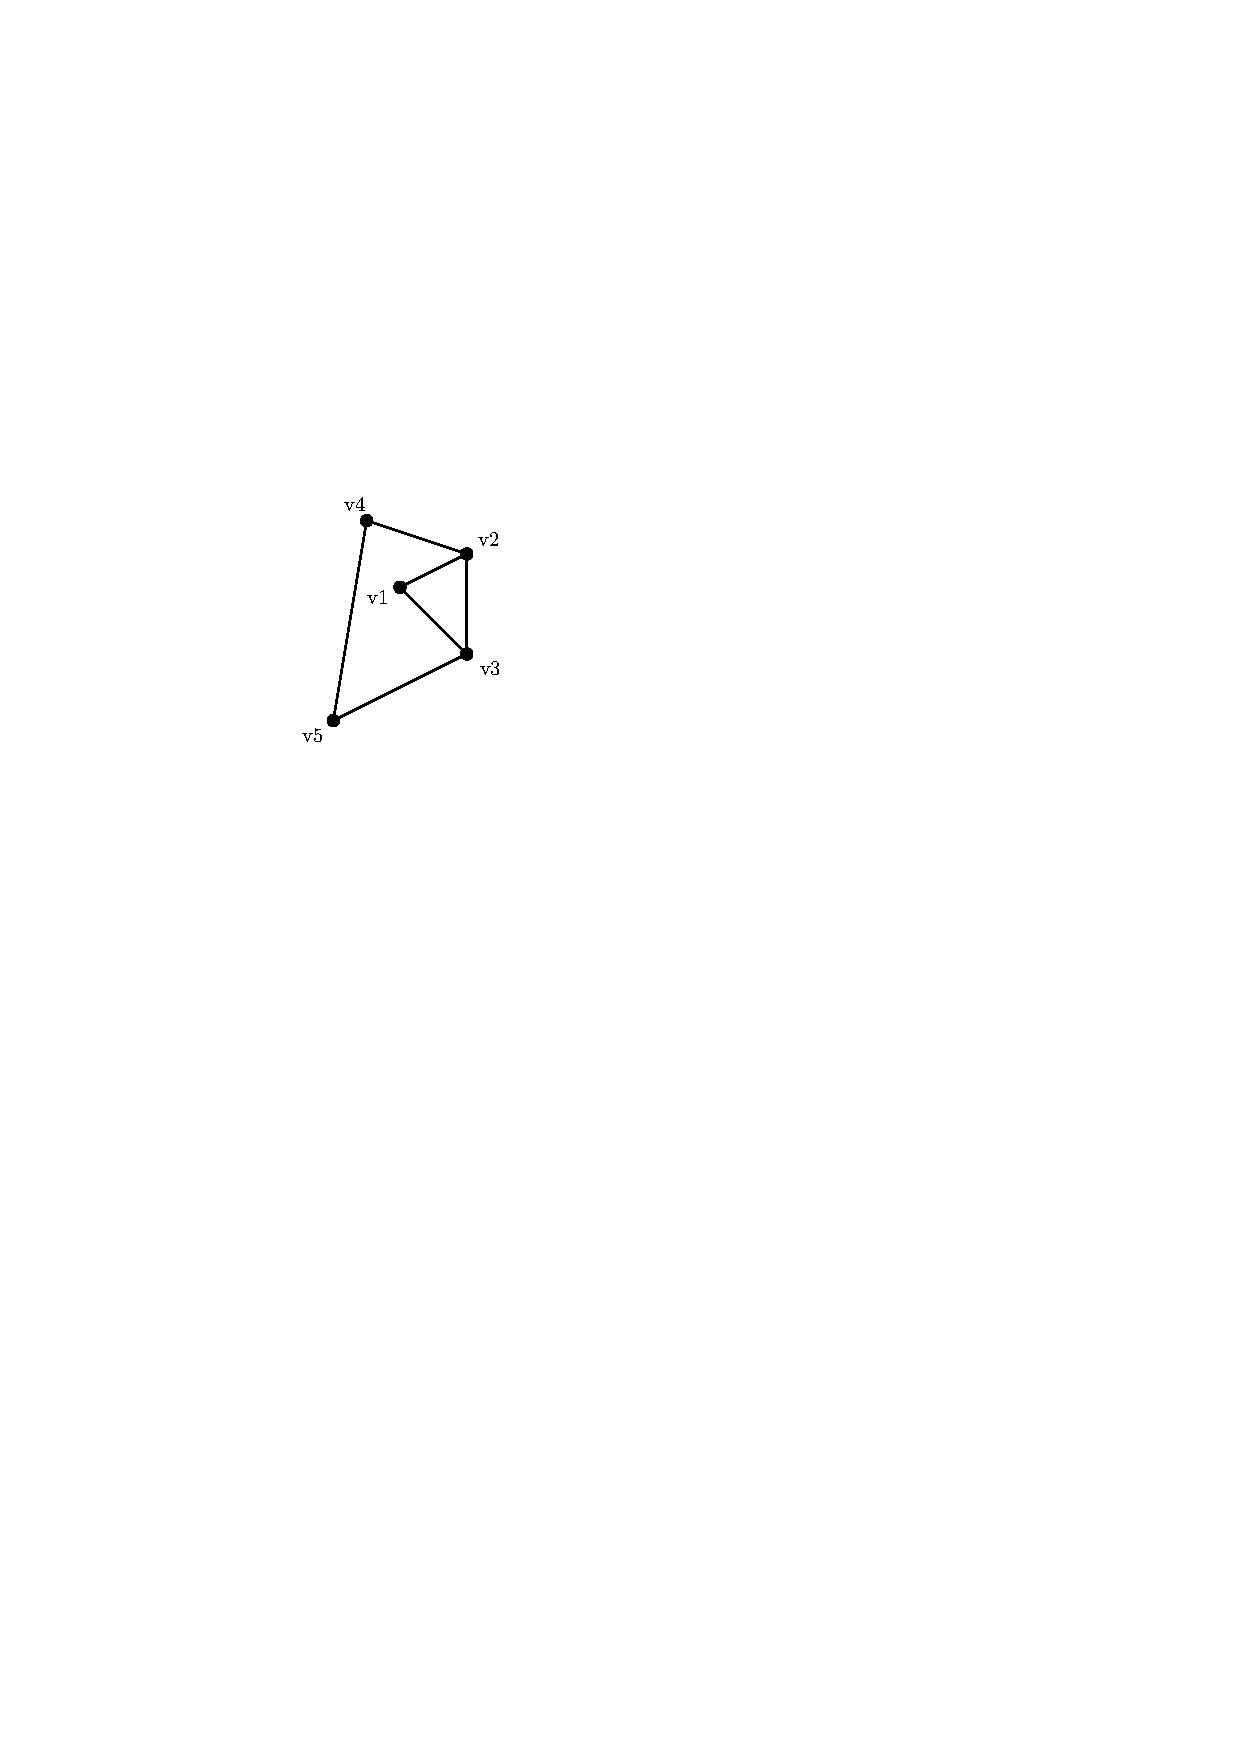
\includegraphics[width = \textwidth]{../media/iso2.pdf} \\
\caption{H}
\label{fig:iso2}
\end{subfigure}
\begin{subfigure}{0.40\textwidth}
\centering
\vspace{0.5cm}
{
\begin{blockarray}{cccccc}
  & v1 & v2 & v3 & v4 & v5 \\
\begin{block}{c(ccccc)}
  v1 & $\ddots$ & 1 & 1 & 0 & 0 \\
  v2 &   & $\ddots$ & 1 & 1 & 0 \\
  v3 &   &   & $\ddots$ & 0 & 1 \\
  v4 &   &   &   & $\ddots$ & 1 \\
  v5 &   &   &   &   & $\ddots$ \\
\end{block}
\end{blockarray}
}
\caption{Adjazenzmatrix von G und H}
\label{mx:iso}
\end{subfigure}
\caption{Zwei isomorphe Graphen G und H}
\label{isoGraph}
\end{figure}

Es sollte nicht vergessen werden, dass ein Graph nicht die räumliche Position der Objekte sondern nur ihre Relation zueinander ausdrückt! Graphen können also komplett unterschiedlich aussehen und dennoch einander entsprechen. Wenn zwei Graphen bei gleichbleibenden Nachbarschaften der Ecken aufeinander abgebildet werden können spricht man von isomorphen Graphen \cite[106]{theory}. Daraus ergibt sich für isomorphe Graphen auch immer eine gleiche Adjazenzmatrix Abbildung (~\ref{isoGraph}).

\subsubsection{Gerichtete Graphen}
Im Gegensatz zu einem ungerichteten Graphen können bei einem gerichteten Graphen Kanten nur in einer Richtung durchlaufen werden. Die Kanten werden daher durch Pfeile anstatt Linien dargestellt. 

$$G = (V,R)$$

Demnach ist auch 
\begin{figure}[h]
\centering
\begin{subfigure}{0.49\textwidth}
\centering
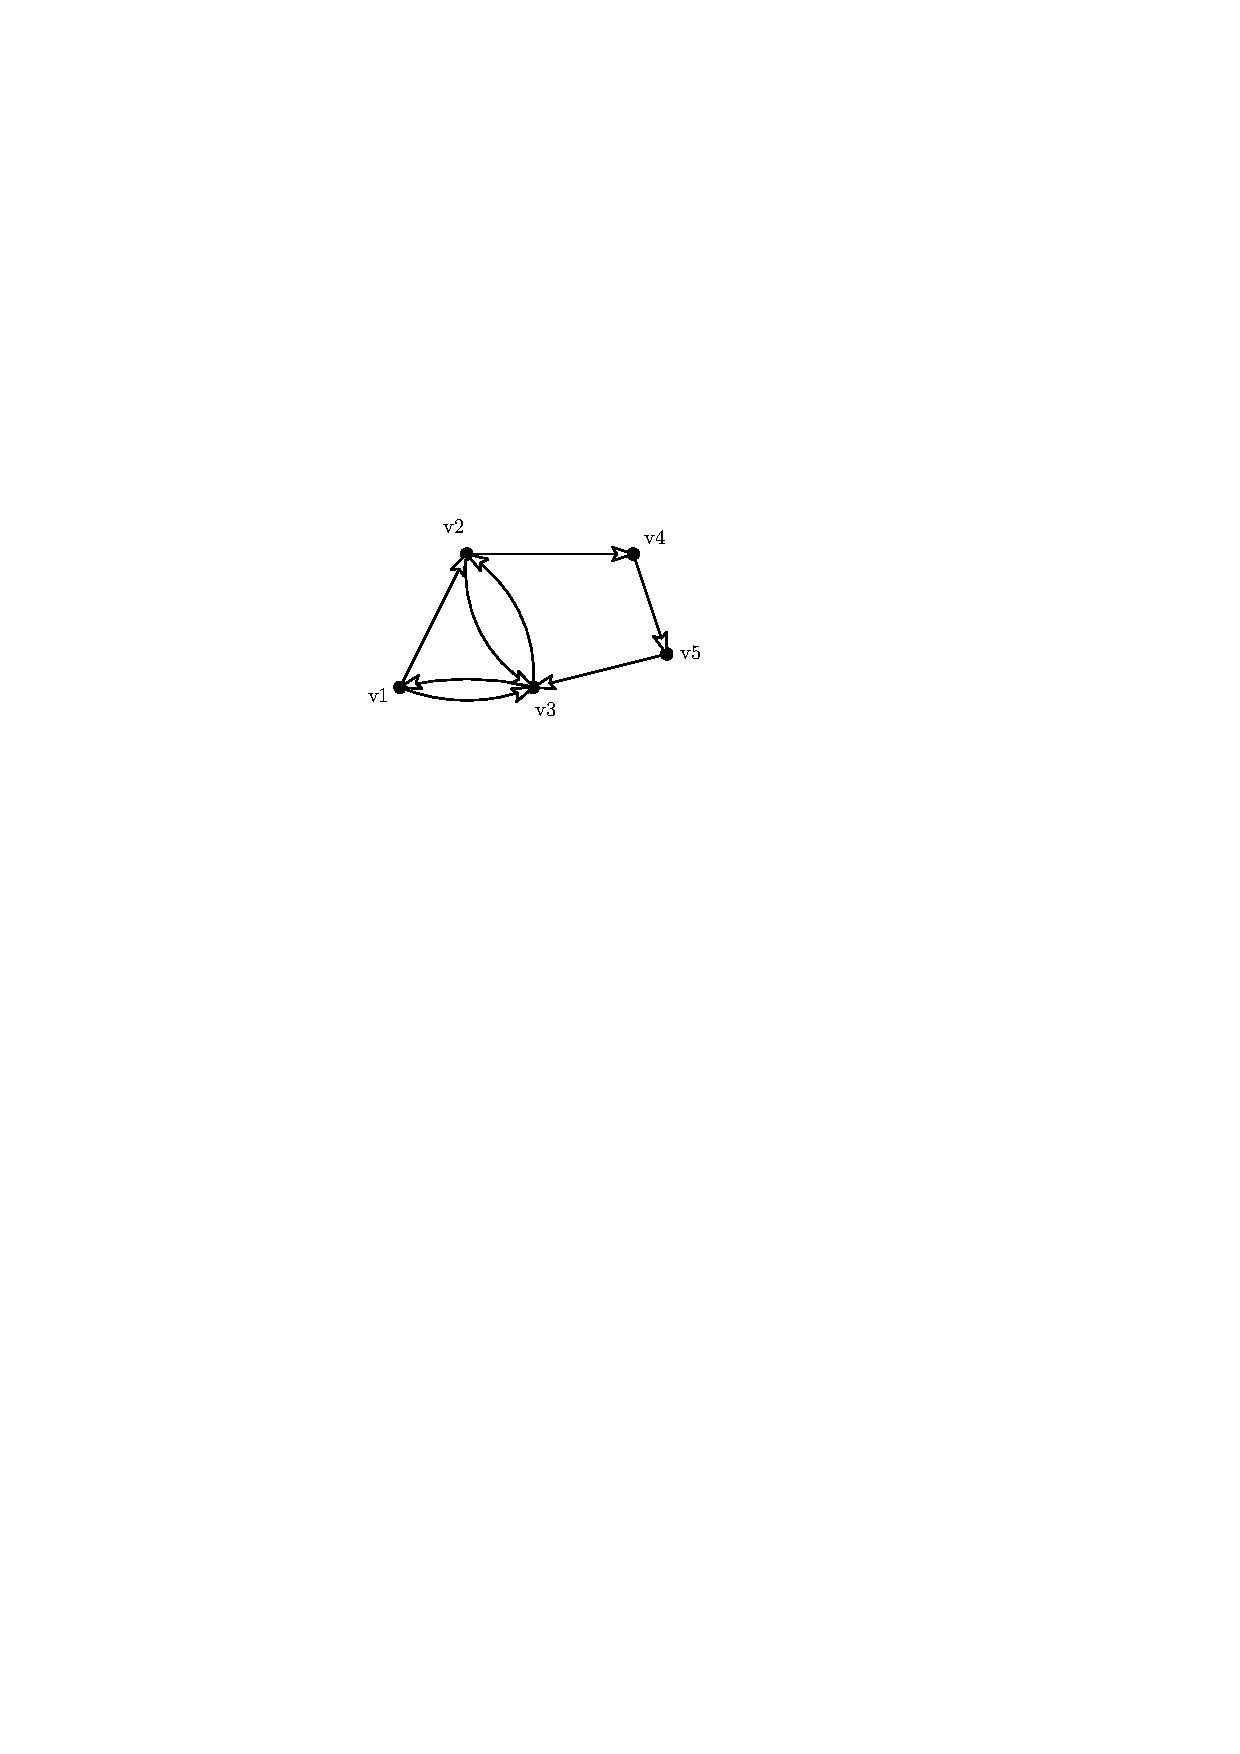
\includegraphics[width = \textwidth]{../media/gerichtet.pdf} \\
\caption{G}
\label{fig:directed}
\end{subfigure}
\begin{subfigure}{0.49\textwidth}
\centering
{
\begin{blockarray}{cccccc}
  & v1 & v2 & v3 & v4 & v5 \\
\begin{block}{c(ccccc)}
  v1 & 0 & 1 & 1 & 0 & 0 \\
  v2 & 0 & 0 & 1 & 1 & 0 \\
  v3 & 1 & 1 & 0 & 0 & 0 \\
  v4 & 0 & 0 & 0 & 0 & 1 \\
  v5 & 0 & 0 & 1 & 0 & 0 \\
\end{block}
\end{blockarray}
}
\vspace{0.1cm}
\caption{Adjazenzmatrix von G}
\label{mx:directed}
\end{subfigure}
\caption{Ein gerichteter Graph G}
\label{directedGraph}
\end{figure}

\subsubsection{Gewichtete Graphen}
In dieser Arbeit bezeichnet der Begriff \textit{gewichteter Graph} einen Kanten-gewichteten Graphen, bei dem jeder Kante ein Wert zugewiesen wird.

$G = (V,E)$ mit $c: R \rightarrow \mathbb{R}$

Neben dem Kanten-gewichteten gibt es auch Knoten-gewichtete Graphen, bei welchen entsprechend die Knoten gewichtet werden. Diese werden aber nur für wenige Problemstellungen gebraucht und sind hier nicht von Belang. Gewichtete Graphen können gerichtet und ungerichtet sein. Ein klassisches Beispiel hierfür ist der Linien-Netzplan einer Bahn, bei dem die Knotenpunkte einzelne Haltestellen darstellen und die Kantengewichte die benötigten Minuten beinhalten.

\begin{figure}[h]
\centering
\begin{subfigure}{0.49\textwidth}
\centering
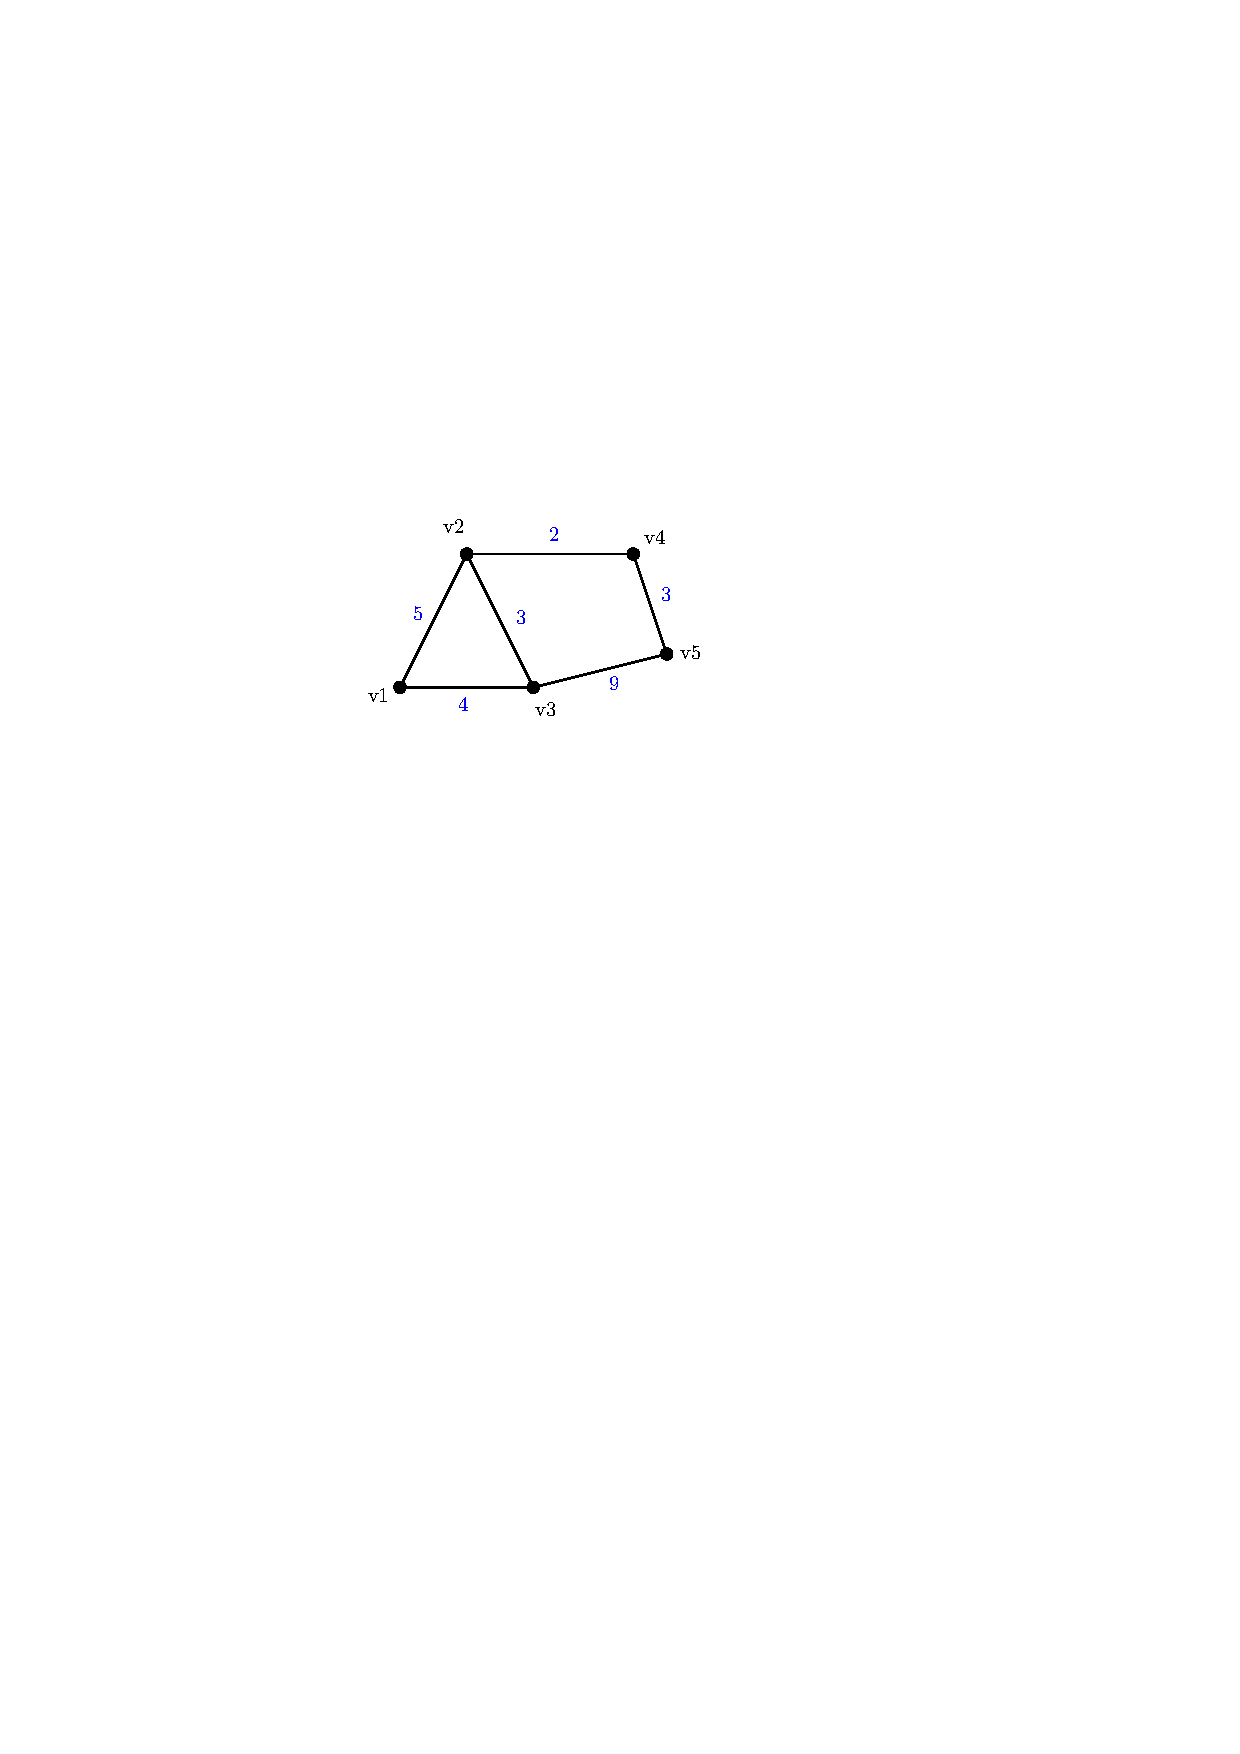
\includegraphics[width = \textwidth]{../media/gewichtet.pdf} \\
\caption{G}
\label{fig:weighted}
\end{subfigure}
\begin{subfigure}{0.49\textwidth}
\centering
{
\begin{blockarray}{cccccc}
  & v1 & v2 & v3 & v4 & v5 \\
\begin{block}{c(ccccc)}
  v1 & 0 & 5 & 4 & 0 & 0 \\
  v2 & 5 & 0 & 3 & 2 & 0 \\
  v3 & 4 & 3 & 0 & 0 & 9 \\
  v4 & 0 & 2 & 0 & 0 & 3 \\
  v5 & 0 & 0 & 9 & 3 & 0 \\
\end{block}
\end{blockarray}
}
\vspace{0.1cm}
\caption{Adjazenzmatrix von G}
\label{mx:weighted}
\end{subfigure}
\caption{Ein gewichteter Graph G}
\label{weightedGraph}
\end{figure}
Mit gewichteten Graphen können diverse Problemstellungen gelöst werden, zum Beispiel die Bestimmung maximaler (Durch-)Flüsse in Rohrsystemen oder das Berechnen kürzester Wege.

\subsubsection{Bau eines Graphen aus OpenStreetMap Daten}
\label{sec:osmgraph}

Die OpenStreetMap(OSM) Datenstruktur und die Struktur eines Graphen sind im Prinzip gleich. Hier werden Punktobjekte als \textit{Nodes}(Knoten) und Linienobjekte wie Straßen als \textit{Ways}(Wege) bezeichnet. Ein Way ist dabei die Verbindung zwischen zwei Nodes. Zusätzlich gibt es \textit{Relations}(Relationen) die einem Set aus Nodes und Ways einen funktionalen Zusammenhang zuschreiben. Für Straßennetze ist dies äußerst hilfreich um zum Beispiel unterschiedliche Segmente eines Autobahnstücks zusammenzufassen oder um Abbiegebeschränkungen an Kreuzungen zu beschreiben (\cite{osmrelation}).

Um aus den OSM Daten einen routingfähigen Graphen zu erhalten müssen zuerst alle benutzbaren Nodes und Ways extrahiert werden. Diese werden anhand ihrer OSM Tags identifiziert. Dazu gehören alle Arten von Straßen und Wegen sowie als befahrbar gekennzeichnet Ways (zum Beispiel asphaltiert aber ohne Straßentyp). Für das Routing sind vor allem Verbindungspunkte wie Kreuzungen, Ab- und Auffahrten etc. und Sackgassen interessant. Daher werden diese \textit{Tower Nodes} aus den importierten Daten ermittelt. Anschließend werden die Straßen anhand der Verbindungspunkte segmentiert. Danach werden die Verbindungen zwischen den Tower Nodes berechnet und anhand der Distanz gewichtet. Das Grundgerüst des eigentlichen Routing-Graphen ist damit erstellt. Einbahnstraßen und Abbiegebeschränkungen werden berücksichtigt und geben die Richtung der Edges an (\cite{osmgraph}). Die Punkte zwischen zwei Tower Nodes nennt man \textit{Pillar Nodes}. Sie werden als \textit{WayGeometry} auf der jeweiligen Edge gespeichert, da sie nicht für den Routing Vorgang benötigt werden (Abbildung ~\ref{fig:tower}). Das Routing ist dadurch um ungefähr das 8-fache schneller (\cite{graphhopper}). Relevante Attribute wie Geschwindigkeit oder Straßentyp werden vereinheitlicht und als \textit{Flags} auf der Edge gespeichert. Diese sind für die individuelle Gewichtung bei der Routenfindung interessant.  (Mehr zu Gewichtung später in Kapitel ~\ref{backendGraphBuild}(\todo{stimmt die reihenfolge max?}). Zuletzt wird der Graph abgespeichert und ist für Routing Abfragen bereit (\cite{osmgraph}). 

\begin{figure}[h]
\centering
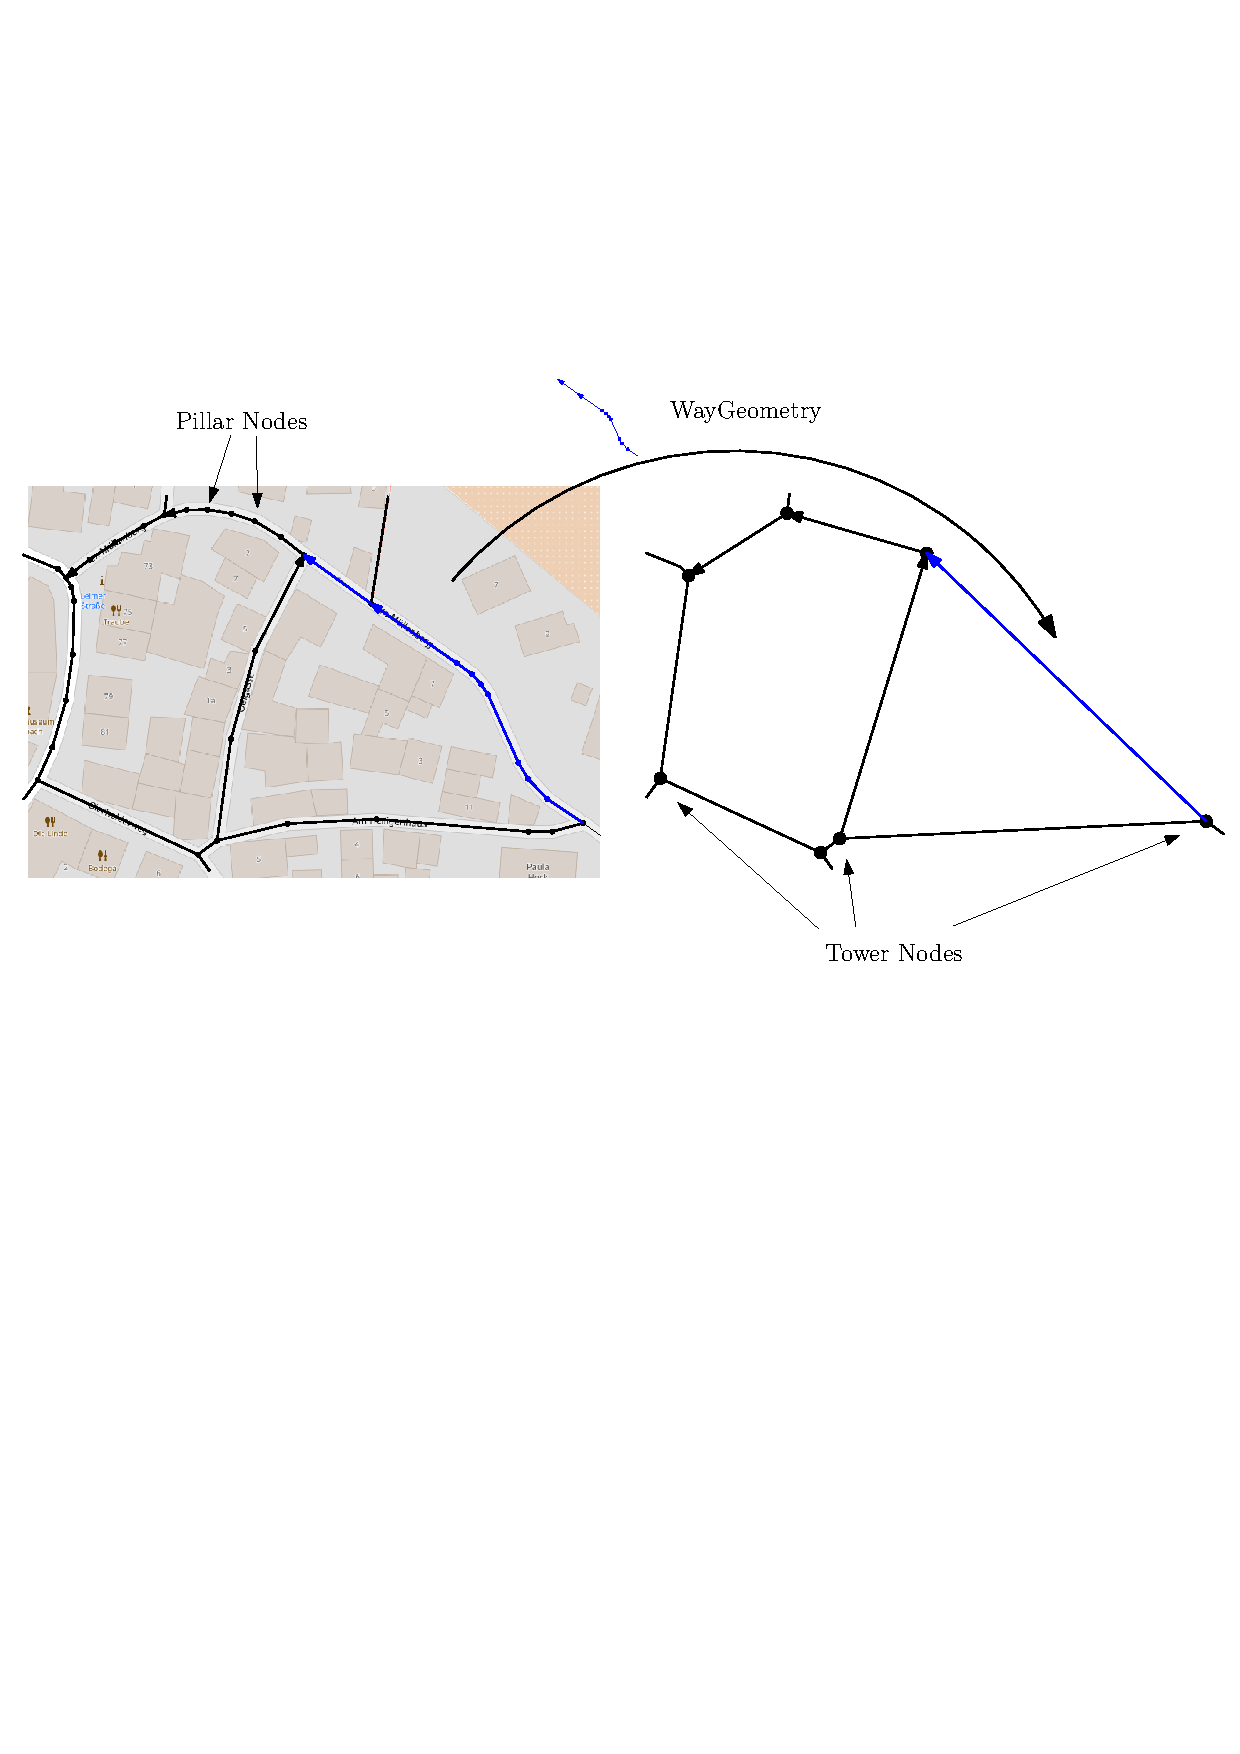
\includegraphics[width = \textwidth]{../media/towers.pdf} \\
\caption{Simplifizierung eines OSM Datensatzes}
\label{fig:tower}
\end{figure}

\subsection{Routing}

Routing bezeichnet den Vorgang in einem Netzwerk Wege zu finden, auf denen Datenpakete entlang gesendet werden können. Diese Definition bezieht sich vor allem auf elektronische Datennetzwerke wie das Telefonnetz oder das Internet. Im Fachbereich der Geo Informations Systeme (GIS) werden hauptsächlich Straßennetze für Routing Analysen verwendet (\cite[165]{handbook}). Ein Weg \textit{P} (\textit{engl: path}) von einem Startnode s zu einem Zielnode z ist eine Folge von benachbarten Ecken mit s als erster Ecke und z als letzter Ecke der Folge (\todo{Abb}).
Die Weglänge entspricht in einem gewichteten Graphen der Summe aller Kantengewichte.

Eine der wichtigsten Netzwerk Analyse Operationen ist die Berechnung des kürzesten Weges zwischen zwei Ecken. Jedes Navigationssystem muss diese Aufgabe erfüllen können. Ein kürzester Weg hat die Eigenschaft, dass die Summe aller Kantengewichte, in anderen Worten die Kosten des Weges, minimal gegenüber allen anderen Wegen ist.

\subsubsection{Shortest Path Problem}
Die nächstliegendste Problemstellung ist das \textit{Shortest Path Problem} welches aber nicht mit dem \textit{Traveling Salesman Problem}(TSP) verwechselt werden sollte. Beim TSP ist die kürzeste Tour auf einem Graphen $G  = (V,E) = K_{n}$\footnote{$K_{n}$ bezeichnet einen vollständigen Graphen bei dem jede Ecke aus V mit jeder anderen Ecke verbunden ist.} mit der Gewichtsfunktion $c: E \rightarrow \mathbb{R}_{+}$ gesucht, die jede des Graphen besucht(\cite[135]{algorithms}).
Das Shortest Path Problem lässt sich in drei Typen untergliedern denen jeweils ein gerichteter Graph $G = (V,R)$ mit der Gewichtsfunktion $c: R -> \mathbb{R}$ zugrunde liegt. Beim \textit{Single Pair Problem}(SPP) ist der kürzeste Weg von einer Ecke a zu einer Ecke b mit $a,b\in V$ gesucht. Das \textit{Single Source Problem}(SSP) möchte den kürzesten Weg einer Ecke a zu jeder anderen Ecke ermitteln (Formel ?). Das \textit{All Pairs Shortest Path Problem}(APSP) sucht den kürzesten Weg von jeder Ecke zu jeder anderen Ecke in V. \cite[169f]{algorithms}

Für ein Routing von Startecke s zur Zielecke z ist das SPP also die richtige Wahl. Allerdings führt die Lösung über das SSP, welches mit dem Algorithmus von Dijkstra gelöst werden kann.

Beispiel:
Ein Anschauliches Beispiel ohne Rechenaufwand für die Lösung des SSPs erhält man, wenn man auf die Karte eines Straßennetzes Fäden auf jede Straße legt. Die Fäden werden an Kreuzungen und am Startpunkt verknotet. Die Fäden stellen den Routing Graph dar. Nun wird der Graph am Startpunkt angehoben. Sofern sich nichts verheddert hat, stellen alle straffen Fäden die kürzeste Route zu den darunter hängenden Knoten dar (\cite[191]{kurt})


\subsubsection{Dijkstra Algorithmus}

 einen gerichteten Graphen $G = (V,R)$ mit einer Gewichtsfunktion $c: R \rightarrow \mathbb{R}_{+}$ \footnote{ohne negative Kantengewichte} sowie eine Startecke $s \in V$. Es gibt eine Warteliste W mit unmarkierten \textit{gesichteten} Ecken v. Dort sind die Kosten für den Weg von s nach v und die jeweilige vorangehende Ecke auf diesem Weg für alle v gepeichert ist. Die Kosten in dieser Liste sind die bisherigen kürzesten Wege für alle v. Sie können sich noch ändern wenn ein noch kürzerer Weg gefunden wird. Diese Liste enthält zu Beginn nur den Startpunkt s mit den Kosten 0. Es gibt eine weitere Liste der kürzesten Wege K in der alle markierten Ecken gespeichert werden.

Dijkstra's Algorithmus (vgl. \cite{dijkstra})markiert die Ecke mit den geringsten Kosten aus W und verschiebt diese nach K. Im ersten Durchlauf ist das die Startecke s. Nun werden alle benachbarten Ecken gesichtet und die Kosten berechnet. Die Kosten und der Vorgänger werden in W gespeichert. Die Ecke mit den geringsten Kosten wird als nächstes markiert, da der Weg dorthin auf jeden Fall ein kürzester ist(vgl. \cite[197f]{kurt}).  Dieser Vorgang wird wiederholt bis alle Ecken aus W markiert wurden und W somit leer ist.

Das Problem bei Graphen mit negativer Gewichtung entsteht, wenn diese auf einer Schlinge oder der Kante eines Rings liegen. Sobald der Algorithmus den Zyklus erreicht, werden die Kosten für die Ecken des Zyklus immer geringer. Die Kosten für den kürzesten Weg nähern sich $-\infty $ während der Algorithmus in einer endlos Schleife läuft. Deswegen ist der Algorithmus nur für positive Kantengewichte anwendbar (\cite[194f]{kurt}).

Damit wurde das SSP gelöst und einen kürzeste Wege zu jeder Ecke des Graphen vom Startpunkt. Daraus ergibt sich auch die Lösung des SPP für den Startpunkt zu jeder anderen Ecke. Es ist jedoch nicht sinnvoll für die Lösung eines SPP jedes mal das SSP für den kompletten Graphen zu berechnen. Das liefert nicht nur viele irrelevante Ergebnisse sondern kostet auch mehr Berechnungsressourcen und Zeit. Daher gibt es unterschiedliche Möglichkeiten den Dijkstra Algorithmus zu beschleunigen.

\subsubsection{Speedup Techniken}

\paragraph*{Early Stopping:}
Der Algorithmus wird jedes mal für den ganzen Graphen ausgeführt obwohl oft nur die Route für einen kleinen Bruchteil des Graphen benötigt wird. Die einfachste Methode ist den Dijkstra zu stoppen, nachdem er den Zielpunkt erreicht hat. 


\paragraph*{Bidirectional Dijkstra:}
Beim bidirectional Dijkstra werden zeitgleich zwei Algorithmen nebeneinander ausgeführt. Einer auf s und einer auf z (auf einem umgekehrt gerichteten Graphen). Für beide Instanzen gibt es eine separate Warteschlange $W_{s}$ und $W_{z}$. Zu Begin wird für jeden Startpunkt die initiale der umliegenden Nodes durchgeführt. Anschließend wird die Ecke mit der geringsten Distanz in beiden Warteschlangen markiert und aus der jeweiligen Warteschlange entfernt. Wird eine Node aus beiden Warteschlangen entfernt, werden $W_{s}$ und $W_{z}$ auf weitere übereinstimmende Nodes geprüft. Für jede Übereinstimmung wird die Distanz in beiden Instanzen Berechnet. Die Node ist Teil des kürzesten Weges wenn die Summe beider Distanzen minimal ist.

\begin{figure}[h]
\centering
\begin{subfigure}{0.30\textwidth}
\centering
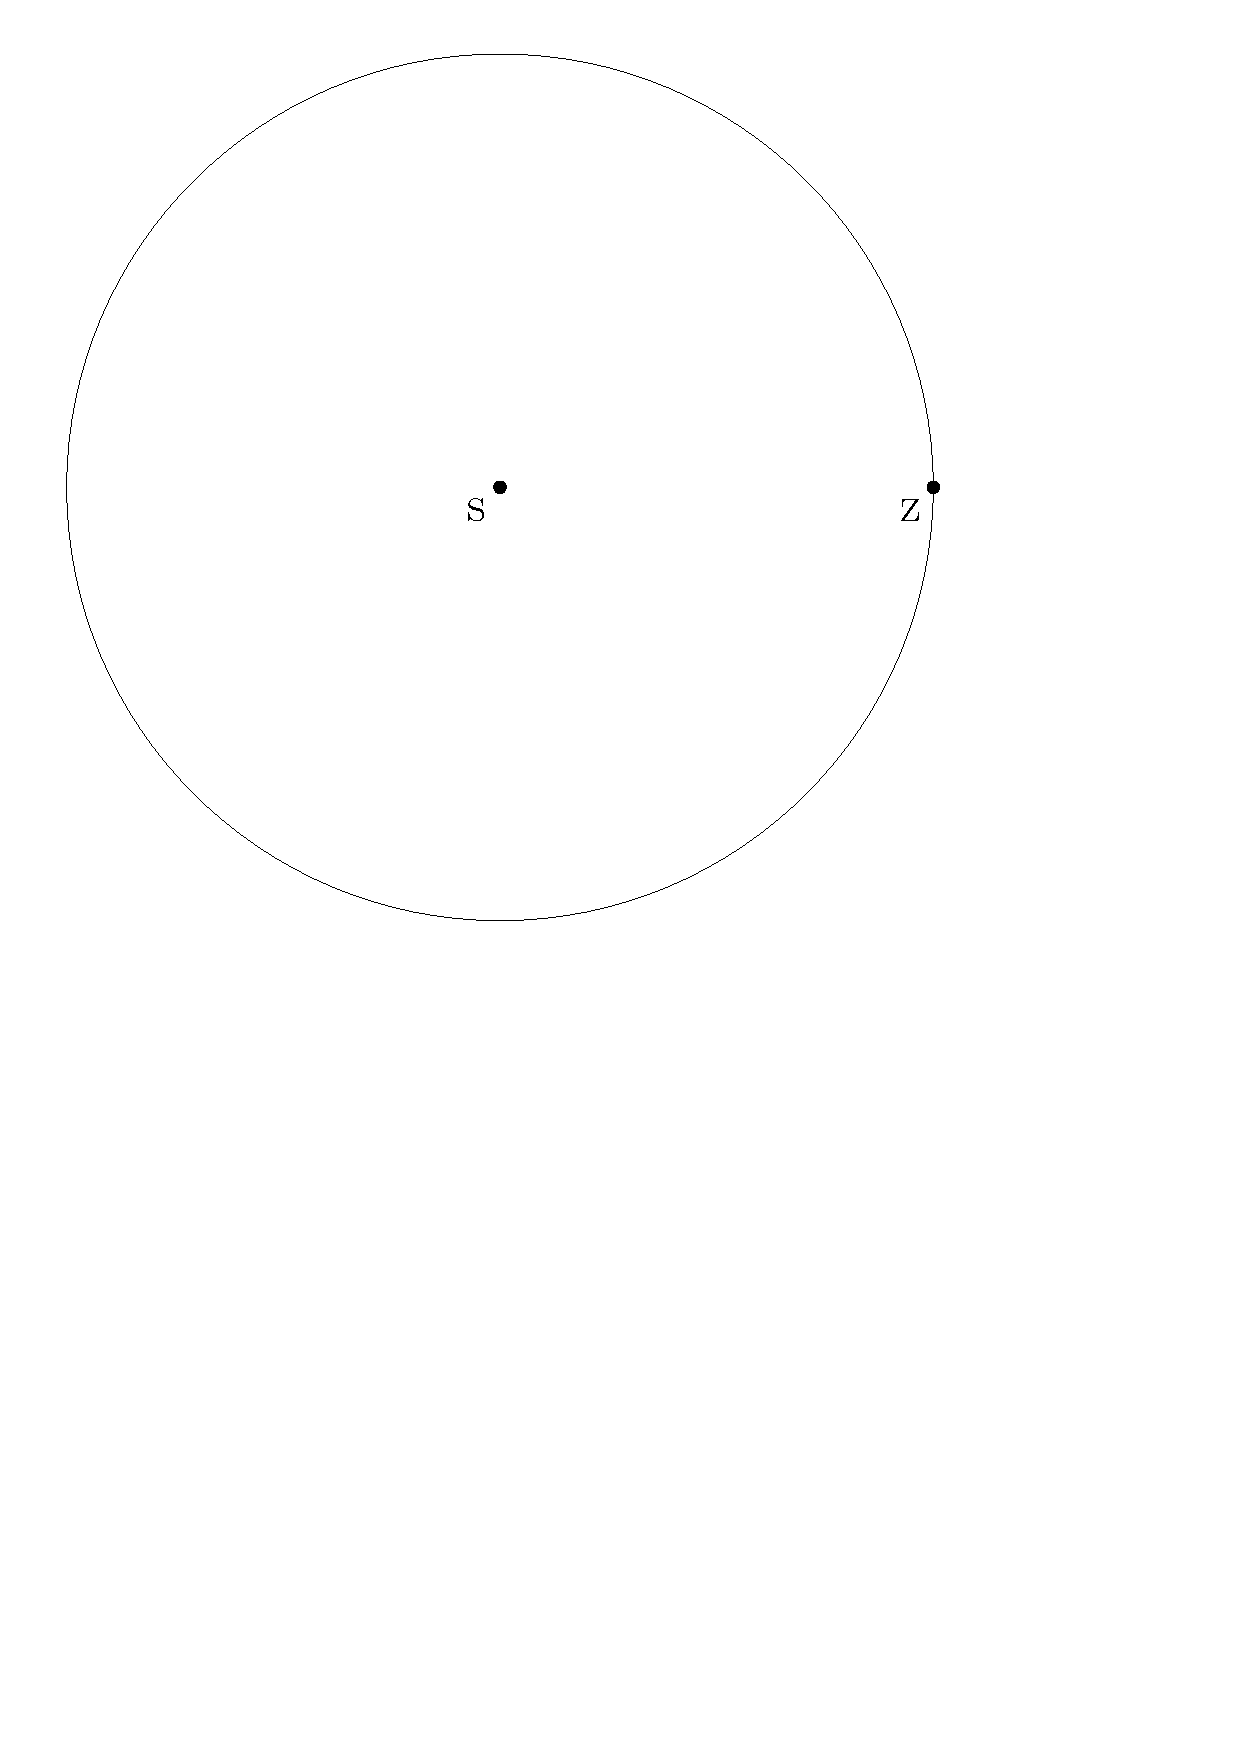
\includegraphics[width = \textwidth]{../media/normaldijkstra.pdf} \\
\caption{Normaler D.}
\label{fig:normalD}
\end{subfigure}
\begin{subfigure}{0.30\textwidth}
\centering
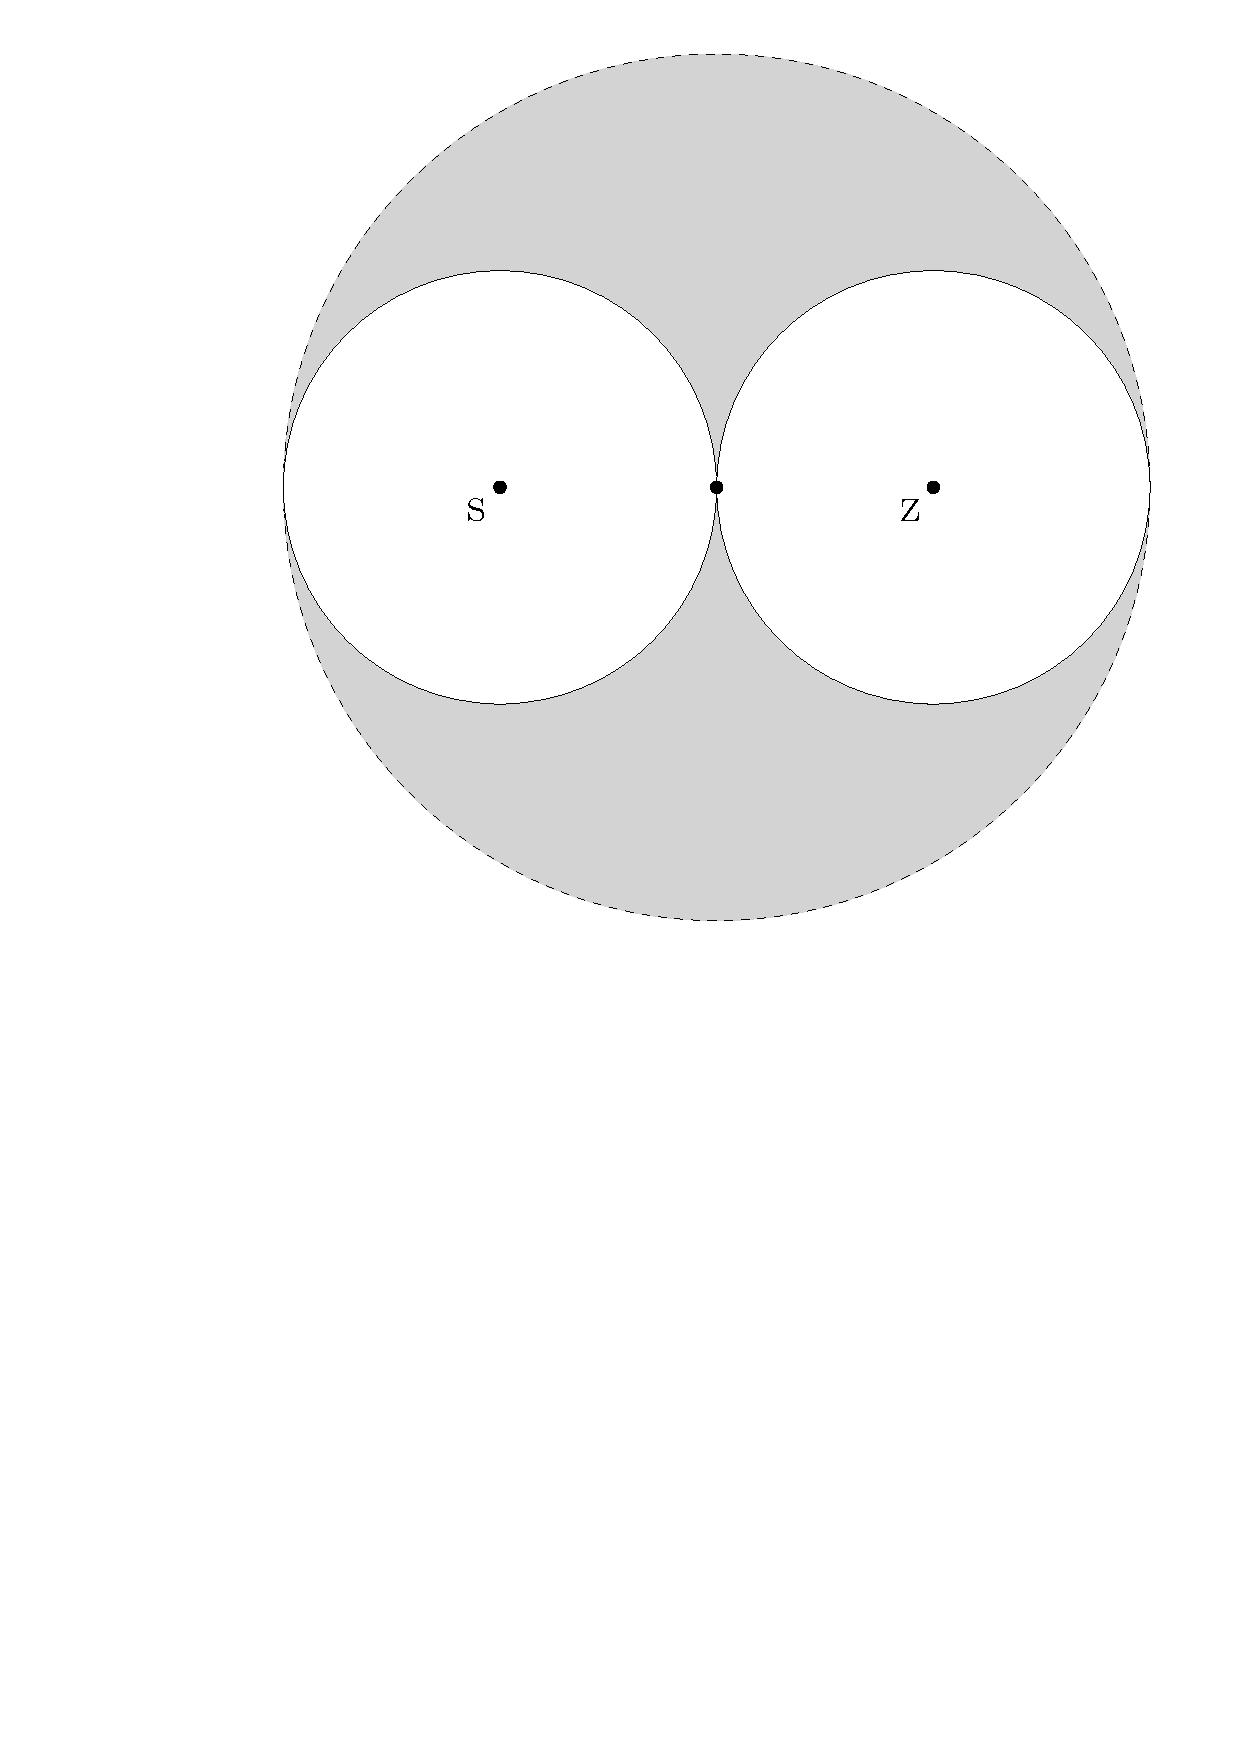
\includegraphics[width = \textwidth]{../media/bidijkstra.pdf} \\
\caption{Bidirectional D.}
\label{fig:biD}
\end{subfigure}
\begin{subfigure}{0.30\textwidth}
\centering
\vspace{1.1cm}
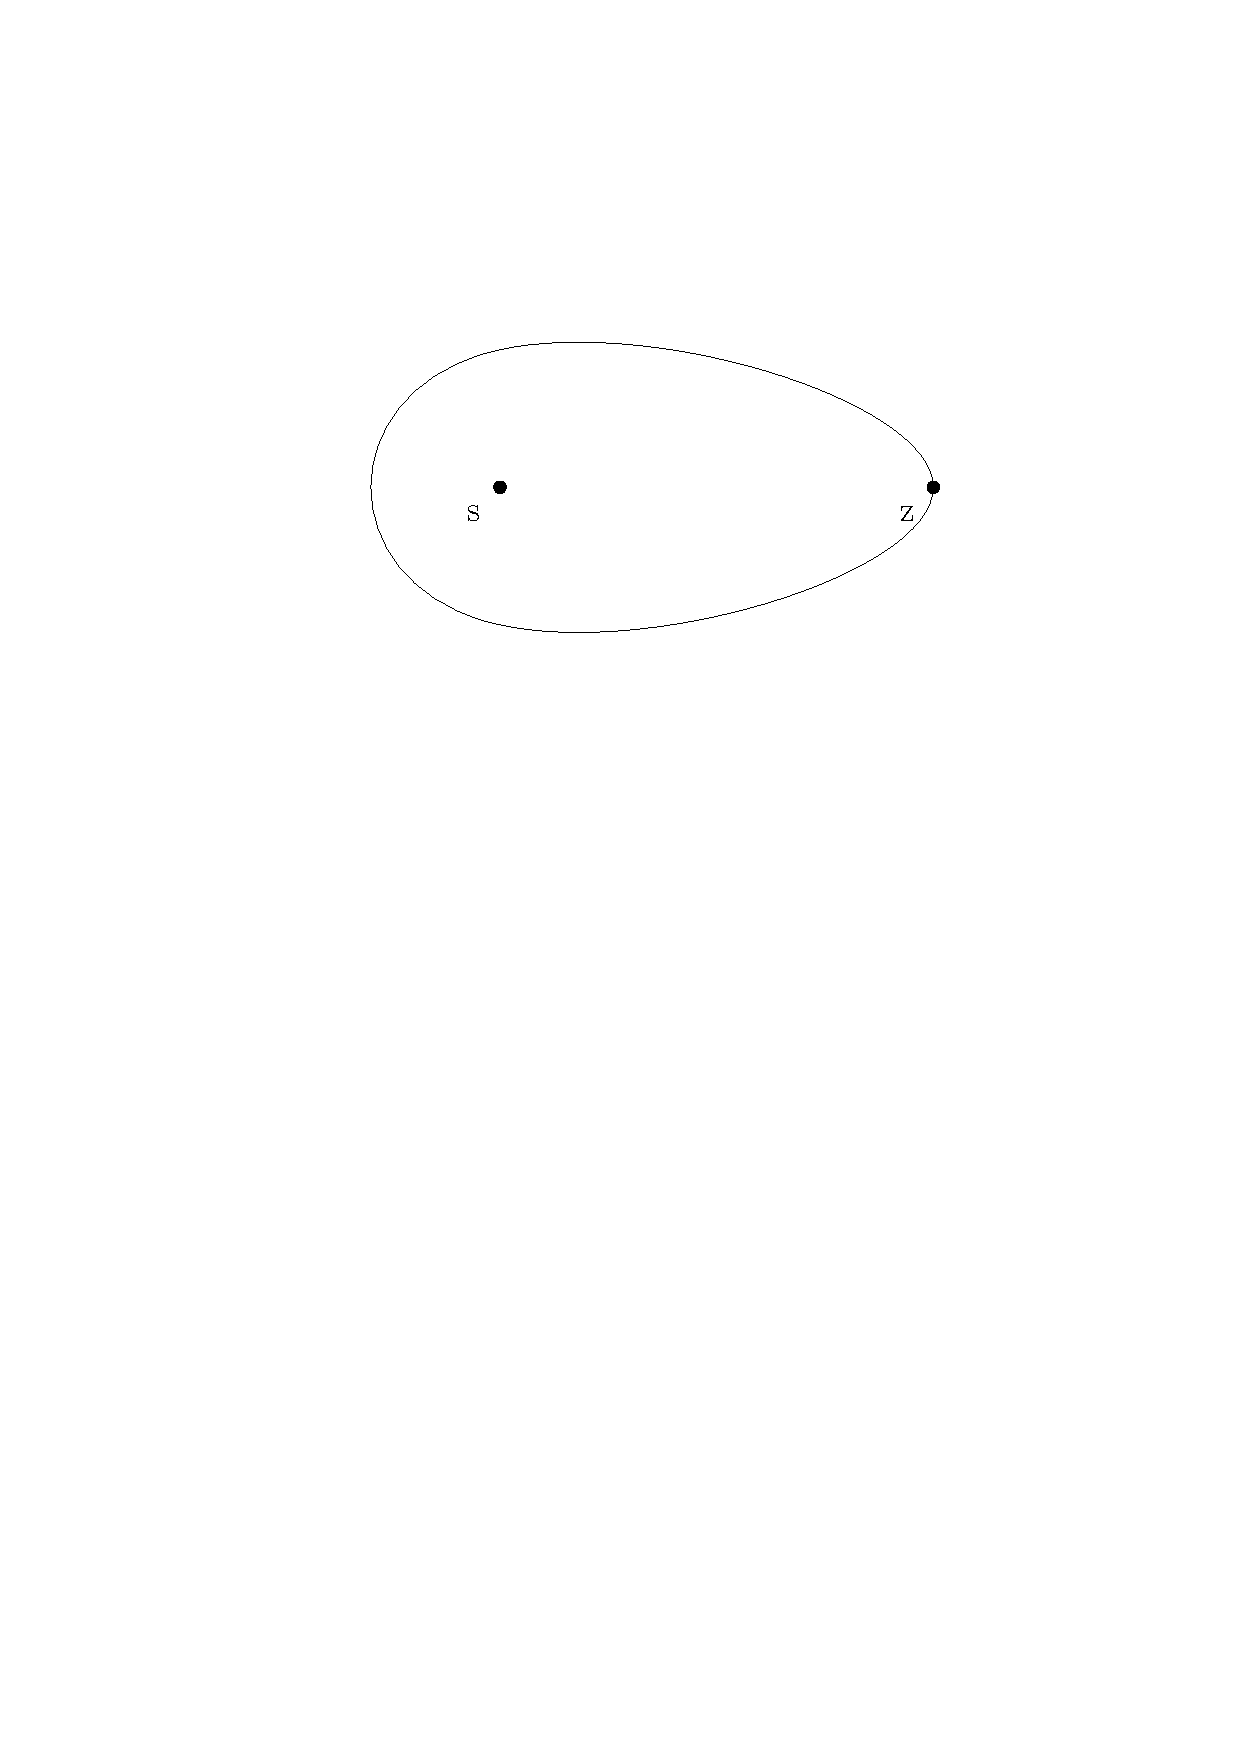
\includegraphics[width = \textwidth]{../media/stardijkstra.pdf} \\
\vspace{0.9cm}
\caption{A*}
\label{fig:starD}
\end{subfigure}
\caption{Speedup Techniken für den Dijkstra Algorithmus}
\label{speedup}
\end{figure}


\paragraph*{A*:}
Der A* Algorithmus ist eine Variante des Dijkstras die den Suchraum in Richtung der Zielecke lenkt. Es wird durch eine Funkiton für jede Ecke die Distanz zum Ziel geschätzt. Diese wird mit den Kantengewichten verrechnet damit Ecken in Zielrichtung früher markiert werden. Die standardmäßig kreisförmige Ausbreitung des Dijkstras wird mit dem A* zu einem Oval gestreckt. Da der Zielpunkt so früher erreicht wird, müssen weniger Iterationen durchgeführt werden.

Diese und weitere Möglichkeiten sind in (\cite[209--213]{kurt}) ausführlich beschrieben.

\subsection{Isochronen Berechnung}

Isochronen sind Linien gleicher Zeit (griech.: \textit{iso} = gleich + \textit{chronos} = Zeit).

Wenn in einem gewichteten Graphen die Kanten die benötigte Zeit enthalten um von einem Knoten zum nächsten zu gelangen, können damit Analysen zur Erreichbarkeit durchgeführt werden. Dazu wird ein SSP für eine zentrale Ecke z mt einem gegebenen Zeitlimit t gelöst. 
Isochronen können mit unterschiedliche Methoden berechnet werden. Das resultierende Objekt ist immer ein Polygon, welches jeden in gegebenem Zeitlimit erreichbaren Punkt beinhaltet.


\subsubsection{Gitterbasierter Ansatz}
Beim \textit{marching squares} algorithmus wird um das Zentrum ein Gitter über dem Graphen gebildet. Die Eckpunkte des Gitters erhalten dabei die Werte des nächsten Punktes auf dem Graphen. Anschließend werden auf den Kanten des Gitters diejenigen Punkte markiert, bei denen der Wert mit dem gesuchten Zeitlimit übereinstimmt. Die markierten Punkte werden verbunden und bilden schließlich die Isochrone.

(Abb. recursive grid / marching squares)

Der Vorteil dieses Algorithmus ist, dass die Maschengröße des Gitters angepasst werden kann. Bei sehr kleinen Maschen liefert der Algorithmus ein sehr genaues Ergebnis. Allerdings werden dabei mehr Ressourcen zur Berechnung gebraucht. Daher können nur kleine Gebiete und geringe Zeitlimits berechnet werden. Bei weiten Maschen ist der Algorithmus dagegen sehr schnell und kann große Distanzen und lange Zeitspannen berechnen. Das Ergebnis ist dementsprechend aber auch ungenauer.

\subsubsection{Dreiecksvermaschung}
\cite{isochrones} beschreiben ein anschauliche Methode um Isochronen zu berechnen. Nach der Lösung des SSPs werden den Ecken des Graphen die geographische Koordinate der repräsentierten Kreuzung zugeteilt. Die Kanten werden nicht benötigt und daher entfernt. Es liegt also eine 3D-Punktwolke vor. Jeder Ecke wird nun die benötigte Zeit zugewiesen, mit der diese zu erreichen ist. Anschließend werden die Ecken nach dem Delaunay Triangulationsverfahren vermascht. Es entsteht eine Art Trichter mit der Startecke als Tiefpunkt auf der Höhe Null. Wird dieser Trichter auf Höhe des Zeitlimits geschnitten, entsprechen von oben betrachtet die Randkanten des Trichters der Isochrone.



\subsubsection{Formenbasierter Ansatz}
Die Implementierung des ORS zur Berechnung von Isochronen verwendet ist ein formen basierter Ansatz. Zuerst werden mit dem in Kapitel .. bereits ausführlich erklärten Dijkstra Algorithmus alle in gegebener Zeit erreichbaren Kanten markiert. Anschließend werden die geographischen Punkte (Pillar Nodes) aus der  WayGeometry der Kante extrahiert (Siehe Kapitel ~\ref{sec:osmgraph} auf Seite ~\pageref{sec:osmgraph}).  Um jeden der extrahierten Punkte wird ein kreisförmiger Pufferbereich gelegt. Dadurch können nahe beieinanderliegende Punkte übersprungen werden. Mit den verbleibenden Punkten wird eine Punktwolke generiert. Auf diese Punktwolke wird nun der alpha shape algorithmus(Zitat) angewandt um die Isochrone als Hülle um die Erreichbaren Wegsegmente zu zeichnen.
(Abb. Pictures shape based stuff)
Mit diesem Ansatz Distanzen bis zu 100km berechnet werden. Je nach Transportmittel entstehen also Unterschiedliche Zeitlimits für die Isochronen Berechnung: Mit dem Auto können bis zu einer Stunde, mit dem Rad bis zu fünf Stunden und zu Fuß sogar bis zu 20 Stunden abgefragt werden. Dieser Ansatz liefert präzise Ergebnisse bei schnellen Berechnungszeiten. Die Verwendung der alpha shape Bibliothek verhindert allerdings die Möglichkeit der Darstellung von nicht erreichbaren 'Löchern' innerhalb der Isochronen.

\newpage
\section{Generierung des Routing-Profils}
Die Grundsätzlichen Überlegungen für 
\subsection{Informations Erhebung}
Fragebogen für Feuerwehr Lützelburg\footnote{Lützelburg ist eine stadt in Bayern}

\subsection{Aufbau graph backend}
\label{backendGraphBuild}

to allow different waytypes we have to accept them while creating the graph (kapitel bla)

weightings 
 different weights for different profiles , apply weights to dijkstra?
 
 for unusable edge -> weighting + unendlich (quelle ???)
 for emergency 
 
speed maps

first tests, feedback from firebrigade
way too far.

calc weight for dijkstra
calc millis for time add up



\subsection{Limitierende Faktoren}

\subsection{Erweiternde Faktoren}

\newpage
\section{Ergebnisse}
\paragraph{
Vergleiche zwischen Firetruck - Emergency Vehicle - Car - Heavy Vehicle
+ exemplarische reale beispiele!
}
\paragraph{
\color{red}
Hier ein paar räumliche Beispiele aussuchen und exemplarisch zeigen (Routing und Isochronen), welche Änderungen das Profil mit sich bringt, einerseits innerstädtisch, andererseits auch außerhalb der Stadt. Denn Änderungen als solches ist bisschen schwierig zu definieren. die Jungs aus Lützelburg fragen, welches Gebiet mit den bereits vorhandenen Profilen wirklich schlechte Ergebnisse bringt und jetzt mit Emergency weitaus realitischere!
}

\newpage
\section{Fazit}

Für diesen Zweck geeignet.
Much more accurate than previous profile. 
Für Allgemeingültigkeit weitere Tests nötig


\newpage
\section{Future Work or Ausblick}

Suche nach Löschwasser quellen um den Zielpunkt ( osm tag emergency=fire\_hydrant )
Beschleunigung, bisher nur Faktor, für genauere Berechnungen exakte Beschleunigungsdaten der Jeweiligen Fahrzeugklasse benötigt. Bremsweg, Kurvengeschwindigkeit, Beschleunigungsweg.
rush hour , Tag und Nacht Unterscheidung (nachts weniger los auf Straßen\/ Fußgängerzonen ...)

\printbibliography

\newpage
\section*{Danksagungen}
\todo{An dieser Stelle möchte ich allen danken.. }

\newpage
\todo{empty last page}
%last page

\end{document}
